\documentclass[11pt]{article}
\usepackage[margin=1in]{geometry}
\usepackage{graphicx}
\usepackage{booktabs}
\usepackage{longtable}
\usepackage{array}
\usepackage{xcolor}
\usepackage{amssymb}
\usepackage{hyperref}
\hypersetup{colorlinks=true,linkcolor=blue,urlcolor=blue,citecolor=blue}

\definecolor{scea}{HTML}{1F7A8C}
\definecolor{ext}{HTML}{E07B39}

\title{\textbf{Section 2 --- Exploring single-cell RNA-seq of immune cells\\
across species}\\[2pt]
\large Curating species for cross-species expression of paralogous TFs}
\author{Paralogous-TF project \quad (iteration 11, computational pipeline)}
\date{2026-06-16}

\begin{document}
\maketitle

\section{Question}
One goal of this project is to evaluate the expression of paralogous transcription
factors (TFs) in immune cells using available bulk or single-cell RNA data, and to
do so \emph{beyond human and mouse}. This note inventories which other species have
single-cell RNA-seq (scRNA-seq) of immune cells (blood, spleen, lymph node, bone
marrow / thymus), starting from the EBI Single Cell Expression Atlas (SCEA) and then
widening to all public resources, and places those species on a time-calibrated
evolutionary tree so the phylogenetic coverage --- and its gaps --- is explicit.

\section{What is in the EBI Single Cell Expression Atlas}
SCEA (the single-cell arm of EMBL-EBI's Expression Atlas) uniformly re-processes
every dataset through one pipeline (SMART-like $\rightarrow$ Kallisto; droplet 10x/
Drop-seq $\rightarrow$ Alevin/Salmon $+$ \texttt{emptyDrops}; downstream
\textsc{Scanpy} for clustering and markers), so matrices are comparable across
studies and species. A live pull of the experiment list
(\texttt{www.ebi.ac.uk/gxa/sc/json/experiments}, saved to
\texttt{inputs/scea\_experiments.json}) returned \textbf{383 experiments across 22
species}. Of these, \textbf{9 are vertebrates}, and only \textbf{5 carry a genuine
immune-cell dataset} (Table~\ref{tab:scea}); the other four vertebrates in SCEA
(marmoset, sheep, chicken, \emph{Xenopus}) contain only non-immune tissues
(embryo, gut epithelium, limb, spinal cord).

\begin{table}[h]
\centering
\caption{Vertebrate species in SCEA and their immune-cell scRNA-seq content.
Immune experiments were counted by matching dataset descriptions against an
immune / haematopoietic keyword set.}
\label{tab:scea}
\begin{tabular}{llrr}
\toprule
Common name & Species & Immune exps. & Total exps. \\
\midrule
\textcolor{scea}{\textbf{Human}}     & \textit{Homo sapiens}          & 44 & 159 \\
\textcolor{scea}{\textbf{Mouse}}     & \textit{Mus musculus}          & 24 & 126 \\
\textcolor{scea}{\textbf{Zebrafish}} & \textit{Danio rerio}           &  6 &  15 \\
\textcolor{scea}{\textbf{Rat}}       & \textit{Rattus norvegicus}     &  2 &   3 \\
\textcolor{scea}{\textbf{Rabbit}}    & \textit{Oryctolagus cuniculus} &  1 &   2 \\
Marmoset                             & \textit{Callithrix jacchus}    &  0 &   1 \\
Sheep                                & \textit{Ovis aries}            &  0 &   1 \\
Chicken                              & \textit{Gallus gallus}         &  0 &   4 \\
Frog (Xenopus)                       & \textit{Xenopus tropicalis}    &  0 &   1 \\
\bottomrule
\end{tabular}
\end{table}

Within SCEA the immune comparison is therefore effectively \textbf{human/mouse-centric},
with \emph{zebrafish} as the single deep outgroup (kidney marrow $=$ the functional
analogue of mammalian bone marrow, plus spleen and blood) and rat/rabbit as thin,
single-study additions (bone-marrow mononuclear phagocytes). Figure~\ref{fig:scea}
shows these on the vertebrate tree.

\begin{figure}[h]
\centering
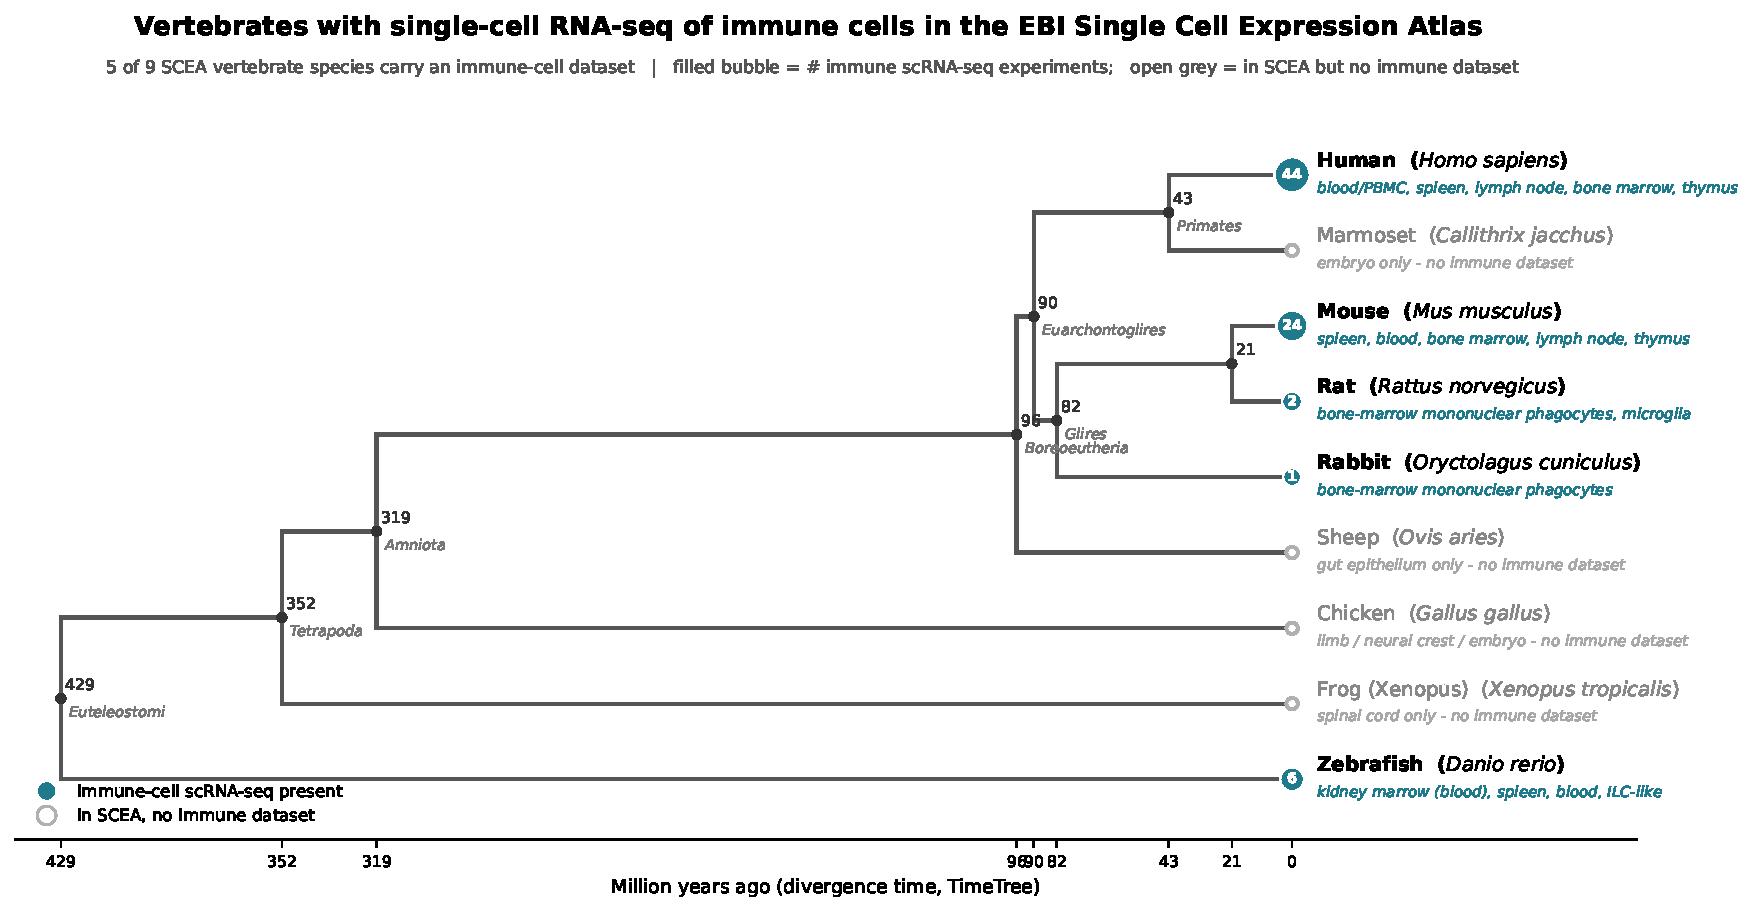
\includegraphics[width=\textwidth]{../results/figures/scea_vertebrate_immune_tree.pdf}
\caption{Vertebrates with immune-cell scRNA-seq \emph{in SCEA}, on a time-calibrated
species tree (present at right). Filled teal bubbles mark species with immune data
(bubble label $=$ number of immune scRNA-seq experiments); open grey tips are in
SCEA but have no immune dataset. Divergence times (Mya) from TimeTree.}
\label{fig:scea}
\end{figure}

\section{The broader cross-resource landscape}
The species that matter most for a cross-species paralog comparison --- non-human
primates and large mammals with secondary-lymphoid-organ coverage --- are
\emph{not} in SCEA; they live in dedicated atlases and papers. Widening to all
public resources adds 14 species (Table~\ref{tab:cross}, Figure~\ref{fig:cross}),
giving \textbf{19 vertebrate species spanning $\sim$429~Myr of evolution}. The
strongest non-human/mouse options with true spleen/lymph-node/marrow coverage are
\textbf{rhesus macaque} (RIRA), \textbf{pig} (porcine lymphoid-organ atlas),
\textbf{cattle} (Cattle Cell Atlas), and \textbf{mouse lemur} (Tabula Microcebus).
Most remaining phylogenetic breadth (carnivores, ungulates, birds) exists only as
\textbf{blood/PBMC} snapshots from cross-species PBMC and livestock studies ---
adequate for circulating-TF expression, thin for tissue-resident immune programs.

\begin{figure}[h]
\centering
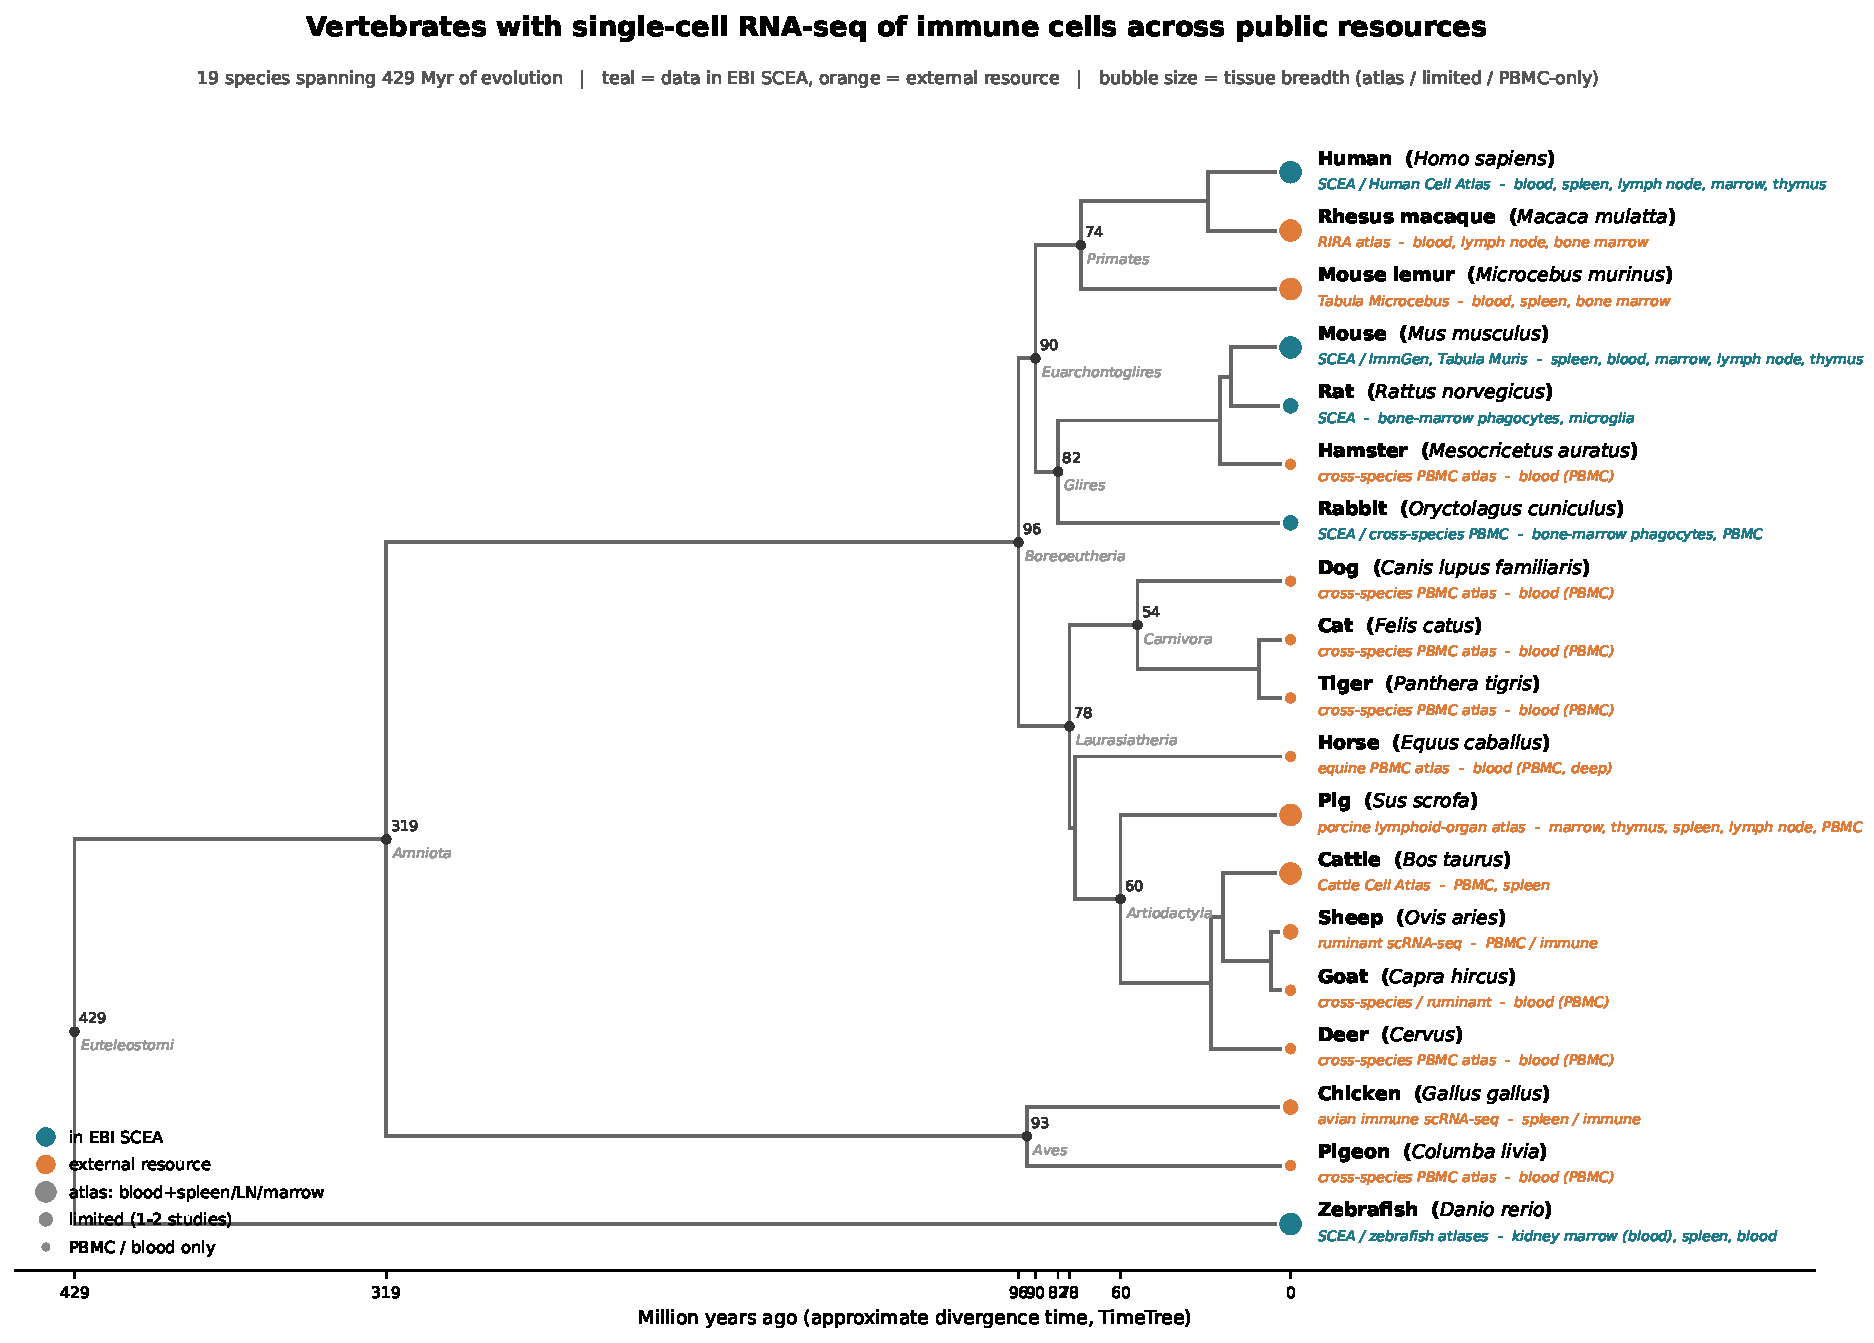
\includegraphics[width=\textwidth]{../results/figures/cross_resource_vertebrate_immune_tree.pdf}
\caption{Vertebrates with immune-cell scRNA-seq across \emph{all} public resources.
Teal $=$ data in EBI SCEA; orange $=$ external resource. Bubble size encodes tissue
breadth: atlas-grade (blood $+$ spleen/lymph node/marrow) $>$ limited (1--2 studies)
$>$ PBMC/blood-only. Divergence times are approximate TimeTree values.}
\label{fig:cross}
\end{figure}

\begin{table}[h]
\centering
\caption{Vertebrate species with immune-cell scRNA-seq across public resources.
``In SCEA'' marks species whose data are in the EBI atlas; ``coverage'' is the
tissue breadth (\emph{atlas} $=$ blood $+$ secondary lymphoid $+$ marrow,
\emph{limited} $=$ 1--2 immune studies, \emph{pbmc} $=$ blood only). The external
set is curated from the literature surveyed and is representative, not exhaustive.}
\label{tab:cross}
\renewcommand{\arraystretch}{1.15}
\begin{longtable}{>{\raggedright}p{2.0cm}>{\raggedright}p{3.0cm}cl>{\raggedright}p{3.2cm}>{\raggedright\arraybackslash}p{3.4cm}}
\toprule
Common & Species & SCEA & Coverage & Resource & Immune tissues \\
\midrule
\endhead
Human & \textit{Homo sapiens} & \checkmark & atlas & SCEA / Human Cell Atlas & blood, spleen, lymph node, marrow, thymus \\
Rhesus macaque & \textit{Macaca mulatta} &  & atlas & RIRA atlas & blood, lymph node, bone marrow \\
Mouse lemur & \textit{Microcebus murinus} &  & atlas & Tabula Microcebus & blood, spleen, bone marrow \\
Mouse & \textit{Mus musculus} & \checkmark & atlas & SCEA / ImmGen, Tabula Muris & spleen, blood, marrow, lymph node, thymus \\
Rat & \textit{Rattus norvegicus} & \checkmark & limited & SCEA & bone-marrow phagocytes, microglia \\
Hamster & \textit{Mesocricetus auratus} &  & pbmc & cross-species PBMC atlas & blood (PBMC) \\
Rabbit & \textit{Oryctolagus cuniculus} & \checkmark & limited & SCEA / cross-species PBMC & bone-marrow phagocytes, PBMC \\
Pig & \textit{Sus scrofa} &  & atlas & porcine lymphoid-organ atlas & marrow, thymus, spleen, lymph node, PBMC \\
Cattle & \textit{Bos taurus} &  & atlas & Cattle Cell Atlas & PBMC, spleen \\
Sheep & \textit{Ovis aries} &  & limited & ruminant scRNA-seq & PBMC / immune \\
Goat & \textit{Capra hircus} &  & pbmc & cross-species / ruminant & blood (PBMC) \\
Deer & \textit{Cervus} &  & pbmc & cross-species PBMC atlas & blood (PBMC) \\
Horse & \textit{Equus caballus} &  & pbmc & equine PBMC atlas & blood (PBMC, deep) \\
Dog & \textit{Canis lupus familiaris} &  & pbmc & cross-species PBMC atlas & blood (PBMC) \\
Cat & \textit{Felis catus} &  & pbmc & cross-species PBMC atlas & blood (PBMC) \\
Tiger & \textit{Panthera tigris} &  & pbmc & cross-species PBMC atlas & blood (PBMC) \\
Chicken & \textit{Gallus gallus} &  & limited & avian immune scRNA-seq & spleen / immune \\
Pigeon & \textit{Columba livia} &  & pbmc & cross-species PBMC atlas & blood (PBMC) \\
Zebrafish & \textit{Danio rerio} & \checkmark & atlas & SCEA / zebrafish atlases & kidney marrow (blood), spleen, blood \\
\bottomrule
\end{longtable}
\end{table}

\section{How to obtain and process the data}
SCEA is fully open (no login). For each experiment, the per-experiment FTP folder\\
\url{https://ftp.ebi.ac.uk/pub/databases/microarray/data/atlas/sc_experiments/<ACCESSION>/}\\
provides MatrixMarket matrices (\texttt{*.aggregated\_filtered\_normalised\_counts.mtx}
$+$ \texttt{.mtx\_rows} gene IDs $/$ \texttt{.mtx\_cols} barcodes), per-cell metadata
(\texttt{*.cell\_metadata.tsv}), clustering (\texttt{*.clusters.tsv}), per-cluster
marker genes (\texttt{*.marker\_genes\_$\langle$K$\rangle$.tsv}), MAGE-TAB sample
metadata (\texttt{*.sdrf.txt}), embeddings, and a ready-made
\texttt{*.project.h5ad} (AnnData) loadable directly with \textsc{Scanpy}. Matrices
are keyed by species-specific Ensembl gene IDs, so the cross-species workflow is:
pick experiments per species, map ETS/paralog orthologs to each species' Ensembl
IDs, then summarise the chosen rows by the supplied cell-type / cluster labels. The
uniform processing means paralog expression patterns can be compared without
re-running quantification. External atlases (RIRA, pig, cattle, Tabula Microcebus)
distribute their own \texttt{h5ad}/Seurat objects via GEO/ArrayExpress/portals.

\section{Implications for the project}
\begin{itemize}
\item For \textbf{tissue-resident} immune expression of paralogous TFs, the usable
species beyond human/mouse are macaque, pig, cattle, mouse lemur, and zebrafish
(deep outgroup) --- all with spleen/lymph-node/marrow coverage and tractable
ortholog mapping.
\item The \textbf{primate axis} is well sampled (mouse lemur $\rightarrow$ macaque
$\rightarrow$ human), which is convenient because ETS-family paralog orthology is
cleanest within primates.
\item Everything else (carnivores, most ungulates, birds) is \textbf{blood/PBMC-only}
--- fine for circulating-cell TF expression, weak for resident programs.
\end{itemize}

\section*{Methods and provenance}
SCEA inventory: \texttt{scripts/05\_scea\_vertebrate\_immune\_tree.py} reads
\texttt{inputs/scea\_experiments.json} (snapshot 2026-06-16), counts immune
experiments per species by keyword, and renders Figure~\ref{fig:scea} with the
table \texttt{results/intermediate/scea\_vertebrate\_immune\_experiments.tsv}
(includes the exact immune experiment accessions). Cross-resource view:
\texttt{scripts/06\_cross\_resource\_immune\_tree.py} renders Figure~\ref{fig:cross}
and \texttt{results/intermediate/cross\_resource\_immune\_species.tsv}. Tree
topology and divergence times are the accepted vertebrate phylogeny with
approximate ages from TimeTree (Kumar et al., \emph{Mol. Biol. Evol.} 2017;
\texttt{www.timetree.org}). The external species set is curated from the surveyed
literature (cross-species PBMC atlas; RIRA; Tabula Microcebus; porcine
lymphoid-organ atlas; Cattle Cell Atlas; equine PBMC atlas) and is representative
rather than a complete database query.

\end{document}
